\documentclass{VUMIFPSkursinis}
\usepackage{algorithmicx}
\usepackage{algorithm}
\usepackage{algpseudocode}
\usepackage{amsfonts}
\usepackage{amsmath}
\usepackage{bm}
\usepackage{caption}
\usepackage{color}
\usepackage{float}
\usepackage{graphicx}
\usepackage{listings}
\usepackage{subfig}
\usepackage{wrapfig}
\usepackage{lithuanian}
\usepackage{longtable}

\usepackage{enumitem}
%PAKEISTA, tarpai tarp sąrašo elementų
\setitemize{noitemsep,topsep=0pt,parsep=0pt,partopsep=0pt}
\setenumerate{noitemsep,topsep=0pt,parsep=0pt,partopsep=0pt}

% Titulinio aprašas
\university{Vilniaus universitetas}
\faculty{Matematikos ir informatikos fakultetas}
\department{Programų sistemų katedra}
\papertype{Kursinis darbas}
\title{Labai panašių neuroninių klasių atskyrimas neuroniniais tinklais}
\titleineng{(Separation of very similar neuronal classes by neural networks)}
\status{3 kurso 5 grupės studentai}
\author{Miglė Vaitulevičiūtė}
\supervisor{dr. Vytautas Valaitis}
\date{Vilnius – \the\year}

% Nustatymai
% \setmainfont{Palemonas}   % Pakeisti teksto šriftą į Palemonas (turi būti įdiegtas sistemoje)
%\bibliography{bibliografija}
\documentclass{article}
\usepackage[backend=biber]{biblatex}
\addbibresource{bibliografija.bib}
\begin{document}
	
% PAKEISTA	
\maketitle
\cleardoublepage\pagenumbering{arabic}
\setcounter{page}{2}

%TURINYS
\tableofcontents

\sectionnonum{Įvadas}



\section{Neuroninis tinklas}
Pagal apibendrintą žmogaus smegenų veikimą buvo sugalvoti neuroniniai tinklai \cite{Goodfellow-et-al-2016}. Bendrai žmogaus smegenys turi šimtus
milijardų neuronų, kurie yra sujungti sinapsėsmis. Per tuos neuronus sklinda elektroniniai impulsai perduodantys informaciją - taip žmonės gali 
atpažinti objektus, garsus ir t.t. Neuroniniai tinklai veikia panašiai. Jie irgi turi daug besijungiančių neuronų, kurie gauna informaciją ir 
pagal tą informaciją gali nuspręsti koks objektas yra paveikslėlyje. Tačiau ties tuo ir baigiasi žmogaus smegenų ir neuroninių tinklų panašumas, 
kadangi neuroniniai tinklai yra kompiuterinė simuliacija - matematinis algoritmas su aritmetiniais kintamaisiais. Ši simuliacija yra suvokiama 
tik žmogui, kuris suprogramavo neuroninį tinklą, pačiam tinklui simuliacija nieko nereiškia, nuovokos neįgauna.

\subsection{Neuroninio tinklo sudėtis}
Neuroninis tinklas yra sluoksnių rinkinys (1 pav.) - neuronų grupė sudaro sluoksnį, kuris yra sujungtas tarpusavyje su kitais sluoksniais. Vienas iš
sluoksnių privalo būti įvesties sluoksnis, kuris atitinkamai pagal užduoti gali gauti įvairios formos informaciją - paveiksliukai, vaizdo
medžiaga, garsas ir t.t. Ši informacija yra reikalinga tam, kad tinklas galėtų ją išanalizuoti ir išmokti. Tuo tikslu, kad vėliau gavęs panašią
informaciją galėtų ją atpažinti - tam reikalingas išeities sluoksnis. Jis yra priešingame neuroninio tinklo gale negu įeities sluoksnis.
Tarp anksčiau apibūdintų sluoksnių yra įvairaus dydžio sluoksnių sistema, kuri atlieka pagrindinį darbą \cite{Woodford-2018}.

\begin{figure}[h]
\centering
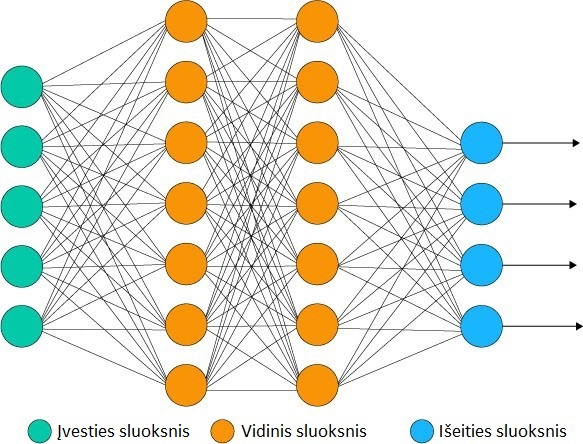
\includegraphics[width=0.5\textwidth]{img/NTSluoksniuSistema.jpeg}
\caption{Sluoksnių rinkinys}
\end{figure}

\subsection{Neuroninio tinklo veikimas}
Jungtys tarp neuronų yra pateiktos skaitine išraiška ir vadinama svoriu. Kuo didesnis šis svoris tuo didesnę įtaką turi vienas neuronas kitam.
Vienam neuronui yra pateikiama visų prieš jį buvusių neuronų informacija ir jungčių svoriai. Kiekvieno neurono informacija yra sudauginama su
jo svoriu ir visi šie duomenys yra sudedami tarpusavyje. Taip iš vektoriaus gaunamas vienas rezultatas ir jei šis rezultatas tinka aktyvavimo
funkcijai, jis yra perduodamas tolimesniems neuronams. Tokio tipo veikimo dizainas yra vadinamas ,,feedforward'' tinklu.

Tačiau jungčių svoriai nėra pastovūs. Kai neuroninis tinklas mokosi, galutinis rezultatas yra lyginamas su tikėtinu teisingu rezultatu, jei šie
rezultatai skiriasi, svoriai yra keičiami atitinkamai tai vadinama ,,backpropagation''. Tokiu būdu yra gerinamas rezultatas ir mažinamas skirtumas
tarp tikėtino ir gauto atsakymų.

\subsection{Aktyvavimo funkcijos}
Aktyvavimo funkcijų yra įvairių, kadangi sprendžiant tam tikrą problemą yra geriau naudoti vienas funkcijas, o kitas problemas - kitas funkcijas.
Pagrinde yra dviejų tipų aktyvavimo funkcijos - tiesinės ir netiesinės. Tačiau tiesinės nėra tokios populiarios, kadangi jos neleidžia įvesčiai
būti lanksčiai. Nors tiesinė funkcija labai dažnai naudojama išeities sluoksnyje.
Netiesinės funkcijos dažniausiai naudojamos vidiniuose sluoksniuose. Šiuo metu labiausiai naudojama yra ReLU, kadangi naudojant šią funkciją mokymo
rezultatai nuolatos gerėja, tačiau ReLU funkcijos spraustumas nesuteikia efektyvumo tinklui \cite{DBLP:journals/corr/XuWCL15}.

Aktyvavimo funkcijos yra skirstomos į:
\begin{itemize}
\item Tiesinė: 
\begin{itemize}
\item Žingsninė (binarinė) - išėjimas yra 0 arba 1.
\end{itemize}
\item Netiesinė: 
\begin{itemize}
\item Sigmoidinė - išėjimas intervale [0; 1].
\item Hiperbolinio tangento - išėjimas intervale [-1; 1].
\item Minkštojo maksimumo - sunormuoja išėjimo vektorių į 1.
\item ReLU - išėjimas intervale [0; begalybė].
\end{itemize}
\end{itemize}


\subsection{Nuostolio funkcijos}
Kai neuroninis tinklas mokosi, jo gaunami rezultatai gali labai skirtis nuo tikėtinų rezultatų. Todėl nuostolio funkcija apskaičiuoja kaip stipriai
skiriasi gautas rezultatas nuo tikėtino. Kuo didesnis nuostolis tuo toliau nuo teisingo atsakymo yra neuroninis tinklas \cite{Cameron-loss-fun}.
Paprasčiausia ir dažniausiai naudojama nuostolio funkcija yra vidutinio kvadrato klaida. Ši funkcija apskaičiuoja kvadratinį skirtumą tarp tikėtino 
ir gauto rezultatų. Tačiau šios funkcijos vienas iš didesnių trūkumų - neproporcingas išskyrimas didelių rezultatų. Kadangi funkcija didėja kvadratiniai,
o ne tiesiniai, kai gaunamas rezultatas tolsta nuo tikėtino rezultato.

Priklausomai nuo to kokią problemą yra bandoma išspręsti yra naudojamos skirtingos funkcijos. Viena iš problemų yra klasifikacijos - dažniausiai išeities
rezultatas yra tikimybės vertė f(x). Bendrai, funkcijos reikšmės dydis parodo gauto rezultato tikslumą. Dauguma klasifikacijos nuostolių funkcijos stengiasi
maksimaliai padidinti tikslumą \cite{clas-loss-2017}. 


Kelios klasifikacijos nuostolio funkcijos:
\begin{itemize}
\item Binarinė kryžiaus entropija.
\item Neigiama registravimo tikimybė.
\item Maržos klasifikatorius.
\item Minkštų maržų klasifikatorius.
\end{itemize}

\subsection{Optimizavimo funkcijos}
Optimizavimo funkcijos naudojamos vidinių tinklo parametrų atnaujinimui, kad sumažinti gaunamų rezultatų netikslumą. 
Visos optimizavimo funkcijos gali būti suskirtytos į du tipus - nuolatinio mokymosi greičio ir prisitaikančio mokymosi.

Nuolatinio mokymosi greičio funkcijos turi hiperparametrą - mokymosi greitį. Jis privalo būti nustatytas, tačiau 
pasirinkti tinkamą mokymosi greitį gali būti sudėtinga - pasirinkus per mažą vidiniai parametrai gali labai lėtai 
konverguoti, o pasirinkus per didelį parametrams gali trukdyti konverguoti ir priversti nuostolio funkciją svyruoti
apie minimumą arba diverguoti. Šio tipo funkcijos turi panašų hiperparametrą - momentą - kuris didina mokymosi greitį, 
kai jis artėja prie minimumo. 

Vienos iš pagrindinių problemų nuolationio mokymosi greičio funkicijų, kad jos privalo turėti nustatytus hiperparametrus 
iš anksto ir jie labai stipriai priklauso nuo modelio ir sprendžiamos problemos. Dar vienas trūkumas, kad toks pats 
mokymosi greitis yra pritaikomas visiems vidinių parametrų atnaujinimams.

Prisitaikančio mokymosi funkcijos turi atskirus kiekvieno parametro mokymosi greičio metodus, kurie teikia euristikos 
metodą, nereikalaujant brangaus darbo rankiniu būdu nustatant hiperparametrus mokymosi greičiui. Tačiau šios funkcijos 
generalizuoja blogiau negu nuolatinio mokymosi greičio funkcijos, nors ir mokymosi metu pasirodo geriau \cite{2017arXiv170508292W}.

% generalization -> http://www.ra.cs.uni-tuebingen.de/SNNS/UserManual/node16.html

% layer types? 
\section{Konvoliucinis neuroninis tinklas}
Konvoliuciniai neuroniniai tinklai yra labai panašūs į paprastus neuroninius tinklus (daugiau informacijos skyriuje ,,Neuroninis
tinklas''). Tačiau pagrindinis skirtumas tarp šių tinklų yra, kad konvoliucinio įeities sluoksnis priima tik tai paveiksliukus, 
kurie jei padaryti su standartine skaitmenine kamera, turi tris komponentus - raudoną, žalią ir mėlyną. Šiuos komponentus galima 
įsivaizduoti kaip tris 2D matricas sudėtas viena ant kitos. Kiekvienos matricos i-osios eilutės ir j-ojo stulpelio elementas 
atitinka nuotraukos pikselį, kurio reikšmė yra intervale nuo 0 iki 255. Kadangi naudojamos informacijos tipas yra specifinis, 
tai labai sumažina tinklo parametrų kiekį ir tinklą padaro efektyvesnį.


Objektų atpažinimas paveiksliukuose yra sudėtingas dėl šių iššukių:
\begin{itemize}
\item Segmentavimas - paveiksliukai gali atvaizduoti įvairias scenas, kuriose gali būti pavaizduota daug objektų, kurie vienas kita gali dalinai uždengti.
\item Šviesa - pikselių intensyvumas gali būti paveiktas šviesos šaltinio ar pačio objekto.
\item Deformacija - objektai gali būti deformuoti įvairiais būdais, pavyzdžiui, kiekvieno žmogaus ranka parašyti skaičiai skiriasi.
\item Galimybės - objektų klasės dažnai nustatomos pagal tai kaip patys objektai yra naudojami, pavyzdžiui, kėdės yra objektai sukurti sėdėti, tačiau jos gali turėti įvairų dizainą.
\item Žvilgsnio taškas - keičiant vietą iš kurios yra žiūrima gali keistis objekto forma, informacija šokinėja per įeities sluoksnio dimensiją (t.y. pikselius). 
\end{itemize}

\subsection{Konvoliucija}
Matematiškam panaudojimui, konvoliucija yra matematinė operacija, kuri apibūdina taisyklę, kuri parodo kaip reikia sujungti du informacijos rinkinius \cite{Convolution-book}. 
Paveiksliukų analizėje, statinė ir pagrindinė funckija yra įeities paveiksliukas, kuris yra analizuojamas, o antroji, judanti funkcija, žinoma 
kaip filtras, nes ji išskiria paveiksliuko ypatybę. Abi funkcijos yra susietos daugyba. 

\\AR REIKIA PAVEIKSLIUKO KURIS PARODYTU KAIP VEIKIA????????????

Tačiau konvoliuciniai tinklai turi daug filtrų, kurie pereina per vieną paveiksliuką, kiekvienas išskirdamas skirtingą paveiksliuko ypatybę.
Pirmuose sluoksniuose šiuos filtrus galima įsivaizduoti kaip horizontalių, vertikalių ar įstrižų linijų filtrus, kurie sukuria paveikslėlio 
kraštų planą. Tinklas paima visus filtrus, gabaliukus paveiksliukų ypatybių vietų, ir juos sudeda į planą, kuris parodo ypatybės vietą. 
Mokydamasis skirtingų proporcijų ypatybių, tinklas leidžia lengvai kurti įvairių dydžių ir greitą ypatybių atpažinimą.

Ypatybių planas yra kontroliuojamas trimis parametrais:
\begin{itemize}
\item Gylis - atitinka filtrų skaičių.
\item Žingsnis - pikselių kiekis, kuris parodo per kiek reikia slinkti filtro matrica per įeities informacijos matricą.
\item Nulių pamušalas - įeities informacijos matrcios kraštus užpilduti nuliais.
\end{itemize}

\subsection{Konvoliucinio neuroninio tinklo sluoksniai}
Neuroniniai tinklai tai yra sluoksnių rinkinys, kuris turi įeities, vidinius ir išeities sluoksnius. Tačiau priklausomai 
kokio tipo neuroninis tinklas vidiniai sluoksniai gali skirtis. Konvoliuciniai neuroniniai tinklai turi tris pagrindinius 
sluoksnių tipus, kurie sudaro vidinį sluoksnį. Šie tipai yra konvoliucinis, sujungimo ir pilno sujungimo sluoksniai.

\subsubsection{Konvoliucinis sluoksnis}
Šis sluoksnis yra pagrindinis konvoliucinio neuroninio tinklo sluoksnis, kuris atlieka daugiausia skaičiavimų.

Kai naudojami paveiksliukai yra nepatogu ir neefektyvu sujungti visus neuronus vienus su kitais. Todėl reikia kiekvieną 
neuroną sujungti su lokaliu įeities informacijos regionu. Šios jungties erdvinė apimtis yra vertinama hiperparametru 
priimtinu lauku, kuris yra lygus filtro dydžiui. Jungties gylio ašis yra visada lygi įeities informacijos gyliui.



\subsubsection{Sujungimo sluoksnis}


\subsubsection{Pilno sujungimo sluoksnis}


\subsection{VGG}
\subsection{Fine-tune}

\section{Ekspermentas}
\subsection{Technologijos}
\subsubsection{ImageNet}
\subsubsection{Keras}

\sectionnonum{Rezultaitai ir išvados}


\printbibliography[heading=bibintoc]  % Šaltinių sąraše nurodoma panaudota
% literatūra, kitokie šaltiniai. Abėcėlės tvarka išdėstomi darbe panaudotų
% (cituotų, perfrazuotų ar bent paminėtų) mokslo leidinių, kitokių publikacijų
% bibliografiniai aprašai. Šaltinių sąrašas spausdinamas iš naujo puslapio.
% Aprašai pateikiami netransliteruoti. Šaltinių sąraše negali būti tokių
% šaltinių, kurie nebuvo paminėti tekste. Šaltinių sąraše rekomenduojame
% necituoti savo kursinio darbo, nes tai nėra oficialus literatūros šaltinis.
% Jei tokių nuorodų reikia, pateikti jas tekste.

\end{document}
